\begin{definition}
    \textbf{Entropię} dyskretnej zmiennej losowej \( X\) definiujemy jako
    \[
        H(X) = \sum_{x \in \im X} -P(X = x) \cdot \lg P(X = x) = \expected{\lg \frac{1}{P(X)}}
    \]
\end{definition}
Zaznaczmy, że w rozdziale o entropii będziemy posługiwać się logarytmem dwójkowym (\( \lg \)), a nienaturalnym (\( \ln \)), tak jak zazwyczaj.

Zdefiniujemy też entropię indykatora (skrzywionego rzutu monetą)
\begin{definition}
    Niech \( p \in (0, 1) \). Definiujemy:
    \[
        H(p) = -p \lg p - (1-p) \lg (1-p)
    \]
    Dla wygody przyjmujemy \( H(0) = H(1) = 0 \).
\end{definition}
\begin{figure}[H]
    \centering
    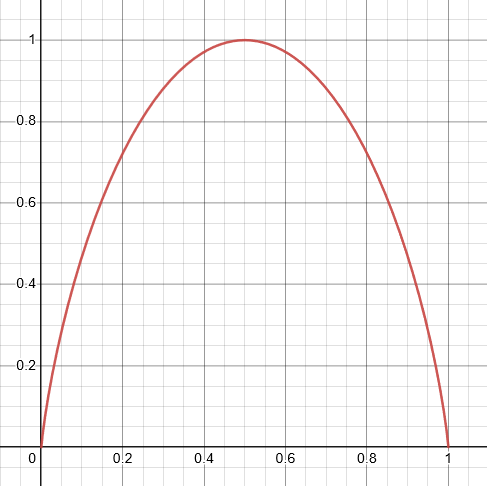
\includegraphics[scale=0.5]{img/entropy/entropy-plot.png}
    \caption{Wykres funkcji \( H \)}
\end{figure}

Widzimy, że entropia jest największa dla \(p = \frac{1}{2} \) -- intuicyjnie odpowiada to faktowi, że sprawiedliwa moneta generuje najwięcej losowości (cały jeden bit informacji), a bardzo skrzywiona moneta bardzo mało (prawie zero bitów informacji). 

Nieco dziwnie jest myśleć o ułamkowych bitach informacji; koncept ten ma więcej sensu jeśli rzucamy taką monetą wiele razy -- jeśli pojedynczy rzut niesie nam pół bitu to 100 rzutów daje nam 50 bitów ,,czystej'' informacji. 

Bardziej namacalne konsekwencje tej intuicji zobaczymy w późniejszych sekcjach, w których pokażemy jak można mierzyć losowość i kompresję za pomocą entropii.

Tym czasem pokażmy inny ciekawy fakt -- jeśli wykonujemy dwa niezależne eksperymenty to łączna entropia takiej zabawy jest sumą entropii każdego z osobna.

\begin{theorem}[Lemat 10.1 P\&C]
    Jeśli \( X_1, X_2 \) są niezależne, oraz \( Y = (X_1, X_2) \) to
    \[
        H(Y) = H(X_1) + H(X_2)
    \]
\end{theorem}
\begin{proof}
    Stety lub nie, jest to jedna wielka pała.
    \[
        H(Y) = -\sum_{x_1, x_2} P\pars{(X_1, X_2) = (x_1, x_2)} \cdot \lg P\pars{(X_1, X_2) = (x_1, x_2)}
    \]
    Z niezależności rozbijamy na iloczyn prawdopodobieństw
    \[
         H(Y) = -\sum_{x_1, x_2} P(X_1=x_1)P(X_2=x_2) \cdot \pars{\lg P(X_1=x_1) + \lg P(X_2=x_2)}
    \]
    Rozbijamy teraz sumę na tej sumie logarytmów:
    \begin{align*}
         H(Y) = &-\sum_{x_1, x_2} P(X_1=x_1)P(X_2=x_2) \cdot \lg P(X_1=x_1) \\
                &-\sum_{x_1, x_2} P(X_1=x_1)P(X_2=x_2) \cdot \lg P(X_2=x_2) 
    \end{align*}
    Zauważamy, że możemy wyciągnąć odpowiednio \( \sum P(X_2 = x_2) \) oraz \( \sum P(X_1 = x_1) \)
    \begin{align*}
         H(Y) = &-\sum_{x_2} P(X_2 = x_2) \sum_{x_1} P(X_1=x_1) \cdot \lg P(X_1=x_1) \\
                &-\sum_{x_1} P(X_1 = x_1) \sum_{x_2} P(X_2=x_2) \cdot \lg P(X_2=x_2) 
    \end{align*}
    Lewe czynniki sumują się do 1, a prawe do odpowiednich entropii, zatem
    \[
        H(Y) = H(X_1) + H(X_2)
    \]
\end{proof}